\documentclass{eceasst}
% This is an empty ECEASST article that can be used as a template
% by authors

% Required packages
% =================
% Your \usepackage commands go here.
\usepackage{orcidlink}
\usepackage{booktabs}
\usepackage{graphicx}
\usepackage{float}

% Use for your first submission the lineno package. Do not forget to remove it for the camera-ready version!!!!
\usepackage{lineno}
\linenumbers

%Mathematical formula accessibility and machine-readability: if you add
\usepackage[accsupp]{axessibility}
\pdfcompresslevel=1
%in the article preamble, you can select an equation and copy-paste it to a text file to recover the TeX math

% PDF accessibility and PDF metadata
\newcommand{\authorRef}[1]{\texorpdfstring{\autref{#1}}{}}
\newcommand{\authorOrcid}[1]{\texorpdfstring{\thinspace\orcidlink{#1}\thinspace}{}}
\newcommand{\geprislink}[1]{\href{https://gepris.dfg.de/gepris/projekt/#1?language=en}{#1}}

\newcommand{\Eg}{E.\,g.}
\newcommand{\eg}{e.\,g.}

% ================================
% Environment for AI Use
% ================================
\newenvironment{aiuse}{%
  \par\vspace{11pt}%
  \noindent\textbf{Declaration on the use of AI:}\enspace}{%
  \par\vspace{11pt}}

% ================================
% Environment for Data availability
% ================================
\newenvironment{data}{%
  \par\vspace{11pt}%
  \noindent\textbf{Data availability:}\enspace}{%
  \par\vspace{11pt}}


% Article frontmatter
% ===================
\title{% Title of the article
GENDERTAGGER: Bridging the Gender Data Gap in Digital Editions through Multi-Method Annotation Workflows}
\short{% Short title of the article (optional)
GENDERTAGGER}
\author{% Authors and references to addresses
Frederike Neuber\authorOrcid{ 0000-0001-8279-9298}\autref{1},
Lou Klappenbach\authorOrcid{0000-0001-6587-3353}\autref{2} and
Tim Westphal\authorOrcid{0009-0000-8580-4558}\autref{3}}
\institute{% Institutes with labels
\autlabel{1} \email{neuber@bbaw.de}\\
\autlabel{2} \email{klappenbach@bbaw.de}\\
\autlabel{3} \email{westphal@bbaw.de}\\
%TELOTA, \url{https://www.bbaw.de/bbaw-digital/telota}\\
TELOTA, Berlin-Brandenburg Academy of Sciences and Humanities}
\abstract{% Abstract of the article
Digital scholarly editions frequently rely on person registers to reconstruct historical networks and contextualize sources. However, gender information in such registers is often incomplete, making structural imbalances within historical datasets difficult to analyze. To address this challenge, we developed genderTagger, a web-based application for semi-automated gender annotation of TEI/XML person registers.\par

The system combines multiple classification approaches, including authority data queries, heuristic methods, statistical models, Transformer-based classifiers, and locally operated language models. Rather than relying on fully automated classification, genderTagger integrates these methods into a human-in-the-loop workflow that supports editorial review, uncertainty-aware decision-making, and direct reintegration into existing TEI/XML workflows.\par

In addition to a tabular annotation interface, the tool provides a gamified mode with score tracking and leaderboards to support collaborative metadata curation. Using the schleiermacher digital edition as a case study, the paper discusses methodological challenges of automated gender annotation in historical corpora, including incomplete authority data, ambiguous naming practices, and algorithmic bias.\par

The project demonstrates how interoperable and uncertainty-aware research software can support Digital Humanities workflows while critically engaging with the limitations of computational gender classification.}
\keywords{% Keywords for the article
gender data gap, digital humanities, digital scholarly editions}


% PDF/A compliance
% ========================
% This is an optional step to help with archiving and long-term preservation
% of electronic documents. It stores XMP metadata, machine-readable content,
% and color profiles in the PDF file. When used, it must appear last in the
% preamble to avoid conflicts with other packages (the pdfx package loads
% hyperref and xcolor).
%\usepackage[a-3u]{pdfx}
%\begin{filecontents}[overwrite]{\jobname.xmpdata}
%\Author{Kim Doe}
%\Title{My Title}
%\Language{English}
%\Subject{Software Science and Technology}
%\end{filecontents}

\begin{document}
\maketitle

% Main part of your article
% =========================

\section{CUT}

%\section{Introduction}
%alte version


Name-based gender classification is a widely used approach in various study fields \cite{buskirk_open-source_2023}. Similar problems have been discussed extensively in adjacent fields such as computational social science and social media research, where scholars have highlighted biases in digital datasets, demographic inference methods, and metadata generation. Research on automated gender detection, for example, has shown that computational approaches often rely on binary classifications and culturally biased name datasets, leading to systematic inaccuracies and exclusions \cite{Karimi Inferring Gender from Names on the Web:
A Comparative Evaluation of Gender Detection Methods}.

Digital scholarly editions as critical representations of historical sources \cite{sahle_digitale_2013} rely heavily on structured metadata and person registers. Such lists of persons serve to gather information about writers of the source itself, but also about people who are mentioned within the edited documents or who stand in some other relation to it. However, they are particularly affected by the gender data gap \cite{criado-perez_invisible_2020}, which does not only concern areas such as medicine or the work environment, but also humanities research. Person registers of digital editions frequently reflect a pronounced imbalance between male and female individuals. This imbalance is rooted partly in the structural asymmetry of the historical sources and their transmission, and partly because existing systems fall short in categorizing person data. Authority files, for instance, frequently lack entries for women and other marginalized persons altogether \cite{aleksander_gendern_2025}.

In most cases, the gender imbalance of digital edition corpora can neither be precisely quantified nor made visible, and editions rarely offer the means to filter or search for persons of a specific gender.\footnote{One example are the biographies in the digital edition \textit{Praktiken der Monarchie}, which allows users to filter entries by gender (female, male, unknown), see Akademienvorhaben Anpassungsstrategien der späten mitteleuropäischen Monarchie am preußischen Beispiel (1786–1918), ed. Berlin-Brandenburgische Akademie der Wissenschaften. Praktiken der Monarchie: Biogramme. Version 9, August 20, 2025. https://actaborussica.bbaw.de/P0006319.} One practical reason why gender metadata is so often absent is scale: the increasing size of digital editions makes manual enrichment of person registers a time-consuming and resource-intensive task. Automated approaches to gender classification based on personal names therefore offer promising possibilities for supporting editorial workflows. However, such approaches remain methodologically challenging in historical contexts, due to ambiguous names, inconsistent spelling variants, incomplete authority data, and the risk of reproducing historical and algorithmic biases. Beyond these technical difficulties, the modelling of gender information is itself a sensitive undertaking. In the context of current societal debates and political backlash around gender, any computational approach must navigate carefully between sensitivity to present-day understandings and the pragmatic realities of categorizing historical persons. 

To address these challenges, we developed genderTagger, a web-based application for semi-automated gender annotation of person registers in digital scholarly editions. Such registers are typically encoded in TEI/XML, where TEI refers to the Text Encoding Initiative, a community standard and vocabulary for the description of historical texts. To assign a gender to a person entry, genderTagger combines multiple classification approaches: authority data queries, heuristic methods, statistical models, Transformer-based models, and local large language models. These methods are embedded within a human-in-the-loop workflow that preserves editorial oversight and supports uncertainty-aware review processes. In addition to a tabular annotation interface, the system also includes optional gamified interaction elements intended to support collaborative annotation workflows.

Using the schleiermacher digital edition\cite{schleiermacher-digital} as a case study, this paper makes the following contributions: it presents a TEI/XML modelling approach for gender annotations that encodes provenance, confidence, and editorial responsibility; it describes and evaluates a multi-method classification pipeline and the inter-method agreement measures used to triage editorial attention; and it reflects critically on the methodological and ethical challenges of computational gender classification in historical corpora.


%%%% alte version: TEI

By “gender” we refer to gender categories historically or culturally associated with personal names within available metadata sources, rather than the self-identified gender of an individual. Eventhough the TEI standard offers both options, we deliberately use the tag \texttt{<gender>} rather than \texttt{<sex>} in our data model, as the classifications generated by genderTagger are derived from socially and historically informed name-gender associations \cite{buskirk_open-source_2023} found in metadata, authority records, and computational models, rather than from biological characteristics. More precisely, the system infers gendered name associations, which may serve as indicators of historically assigned or socially perceived gender categories, but cannot be understood as definitive statements about a person’s identity. Nevertheless, within many historical datasets, name-based classification remains one of the few scalable approaches currently available for making structural gender imbalances and the gender data gap visible.

Therefore, we explicitly record these annotations as assigned or inferred categories in order to preserve transparency regarding their computational and editorial origin. This distinction is particularly important in the context of historical datasets, where the individuals concerned can no longer be consulted regarding their gender identity and where available metadata is often incomplete, ambiguous, or shaped by historical biases. 

Accordingly, the annotations are intended as operational metadata categories for the analysis of structural representation within historical corpora, rather than definitive statements about personal identity.

Annotations are written into the source register as a TEI \texttt{<gender>} child element of \texttt{<person>}, inserted after the last \texttt{<persName>} and before any \texttt{<birth>}, \texttt{<death>}, or \texttt{<note>} children. We deliberately encode the result as an element rather than as the shorthand \texttt{@gender} attribute on \texttt{<person>}: only an element gives us a place to attach the provenance attributes (\texttt{@evidence}, \texttt{@resp}, \texttt{@cert}) that the rest of this section relies on, and only an element can later be extended with a date range, a source pointer, or alternative readings.

\begin{verbatim}
<person xml:id="S0001126">
   <persName type="reg">
      <surname>Arnold</surname>
      <forename/>
   </persName>
   <gender value="female" evidence="assigned"
            resp="#gendertagger" cert="low"/>
   <note>Lehrerin in <placeName key="S0000357">Gnadenfrei</placeName>
   </note>
</person>
\end{verbatim}


The four attributes carry the editorial semantics of the annotation:

\begin{description}
  \item[\texttt{@value}.] The currently supported classification values are \texttt{male} or \texttt{female}; entries the pipeline cannot resolve to one of these (\texttt{unknown}, \texttt{institution}, or empty) receive no \texttt{<gender>} element at all.
  \item[\texttt{@evidence}.] Fixed to \texttt{assigned}, indicating that the annotation represents a historically or computationally assigned category rather than a self-identification of the referenced person. 
  \item[\texttt{@resp}.] The entity responsible for the annotation: \texttt{\#gendertagger} for entries left in the state produced by the automated pipeline, and a human-editor identifier (\eg{} \texttt{\#abc}) for entries that were verified or corrected through the review interface. The same TEI mechanism that records human responsibility statements is reused, redirected at software where appropriate.
  \item[\texttt{@cert}.] Confidence is reduced to two levels, \texttt{high} or \texttt{low}. Human-reviewed entries are always \texttt{high}; automated entries inherit the certainty tier produced by the aggregation step (\S\ref{sec:aggregation}), with the unanimous/strong agreement tiers mapped to \texttt{high} and the single-method tier mapped to \texttt{low}.
\end{description}

The elements and attributes \texttt{<gender>}, \texttt{@cert}, and \texttt{@resp} are standard TEI elements \cite{tei_consortium_tei_2025, beshero-bondar_revising_2024}, applying them systematically to machine-generated annotations makes the resulting data filterable: downstream queries can target \emph{all entries classified female with high confidence} or, equally, \emph{all uncertain entries requiring human review}. This makes machine-generated annotations transparent, queryable, and reviewable within existing editorial workflows.

While TEI itself does not prescribe a fixed taxonomy for gender values, the current implementation adopts a deliberately small controlled vocabulary limited to male and female in order to remain interoperable with existing editorial workflows and authority data sources. The element-based modelling nevertheless allows future extensions with additional or project-specific categories.

Our pipeline uses four output categories: \texttt{male}, \texttt{female}, \texttt{uncertain}, and \texttt{institution}. The binary main classification reflects what name-based methods can in principle resolve --- a statistical association between historical name forms and implied gender. Non-binary, trans, and agender identities are not addressable from name strings alone and are deliberately not represented as classifier output categories.



\begin{figure}[H]
  \centering
  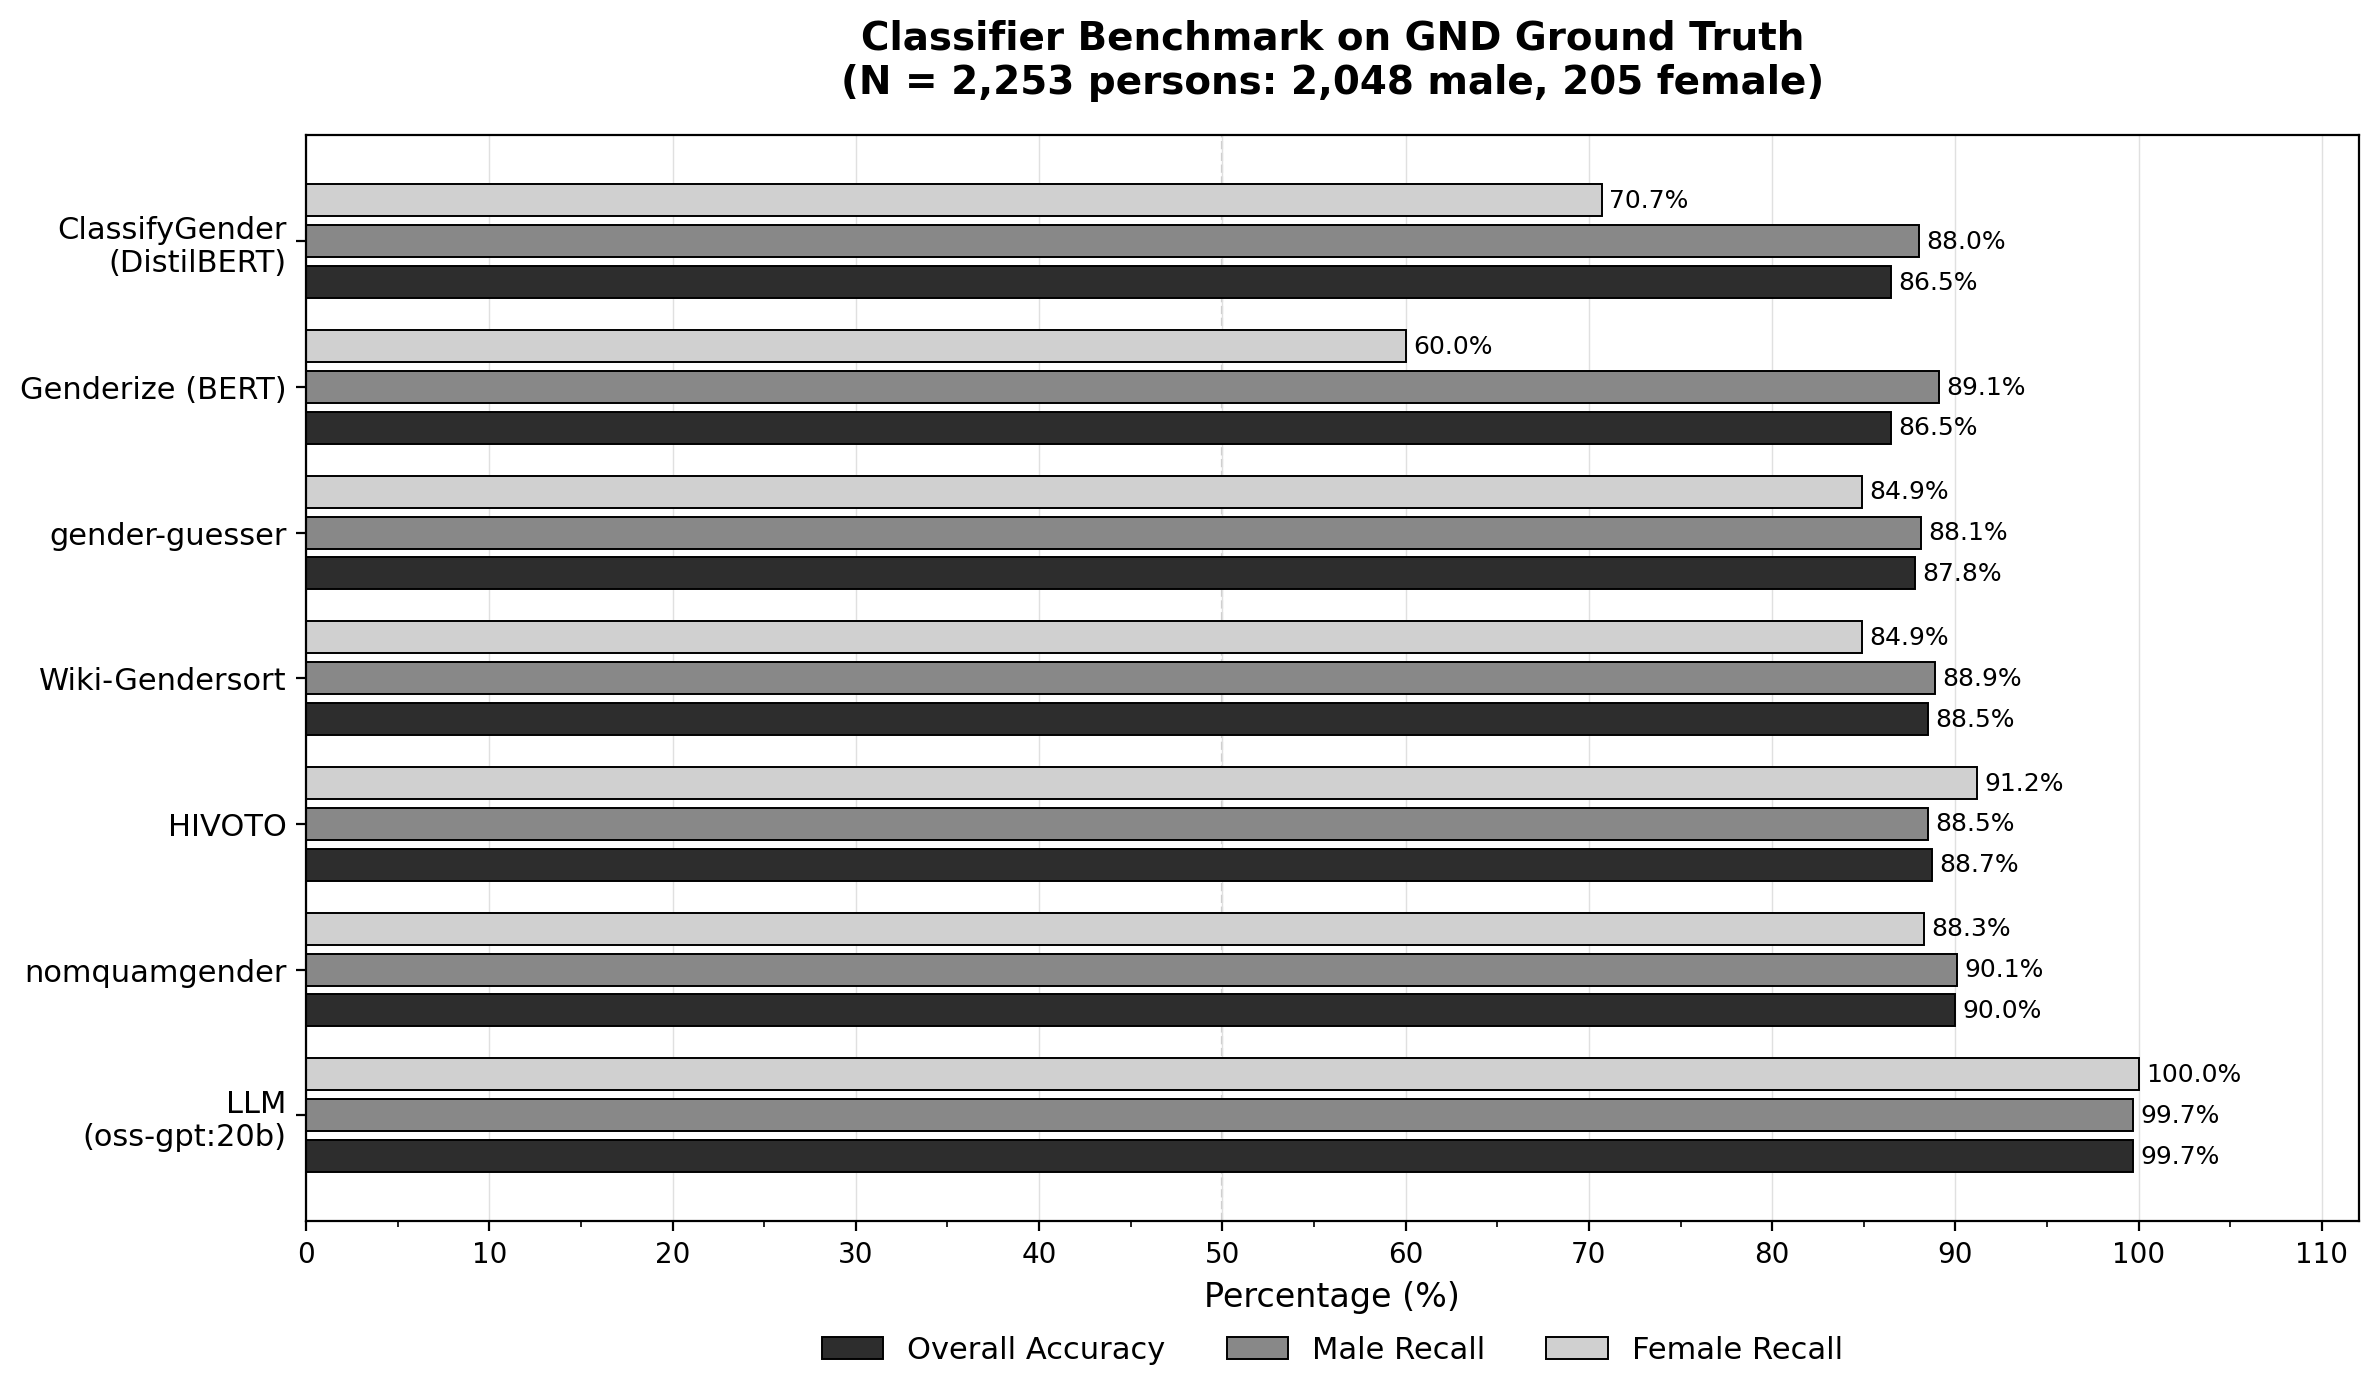
\includegraphics[width=\linewidth]{figures/benchmark_recall.png}
  \caption{Per-method effective accuracy and per-class recall on the Schleiermacher GND benchmark subset ($N = 2{,}253$ persons; $2{,}048$ male, $205$ female). Effective accuracy counts abstentions as errors, which is why the transformer classifiers --- despite high precision when they do answer --- score below the dictionary methods. The female-recall column shows the largest spread between methods.}
  \label{fig:benchmark-recall}
\end{figure}


\begin{table}[h]
  \centering
  \scriptsize
  \setlength{\tabcolsep}{4pt}
  \begin{tabular}{lrrrrrrrr}
    \toprule
     & HV & HV-XGB & NQG & GG & WGS & HF-gz & LLM & HF-DB \\
    \midrule
    HIVOTO          & ---  & 0.89 & 0.88 & 0.85 & 0.86 & 0.63 & 0.73 & 0.69 \\
    HIVOTO-XGB      &      & ---  & 0.88 & 0.82 & 0.83 & 0.67 & 0.77 & 0.73 \\
    nomquamgender   &      &      & ---  & 0.87 & 0.82 & 0.62 & 0.75 & 0.69 \\
    gender-guesser  &      &      &      & ---  & 0.87 & 0.64 & 0.70 & 0.71 \\
    Wiki-Gendersort &      &      &      &      & ---  & 0.70 & 0.70 & 0.76 \\
    HF BERT-gz      &      &      &      &      &      & ---  & 0.56 & 0.80 \\
    LLM             &      &      &      &      &      &      & ---  & 0.62 \\
    HF DistilBERT   &      &      &      &      &      &      &      & ---  \\
    \bottomrule
  \end{tabular}
  \caption{Pairwise Cohen's $\kappa$ values underlying Figure~\ref{fig:kappa-heatmap}. HV~=~HIVOTO, NQG~=~nomquamgender, GG~=~gender-guesser, WGS~=~Wiki-Gendersort, HF-gz~=~HuggingFace BERT-genderize, HF-DB~=~HuggingFace DistilBERT.}
  \label{tab:kappa-matrix}
\end{table}




%discussion



We deliberately did not collapse the methods into a single black-box ensemble. The per-method labels are kept alongside the combined result in the aggregated table, both because editors gain useful epistemic signal from the agreement pattern --- nine methods agreeing on \emph{female} is qualitatively different from five against three with the LLM dissenting --- and because the labels can be re-aggregated under a different combination strategy without re-running the underlying classifiers. The latter matters in practice for the slow methods: re-running the local LLM over several thousand entries takes hours, while changing the voting rule takes seconds.

% [FEHLT: alternative gewichtete Kombinationsstrategien (z.\,B. nach Per-Method-Genauigkeit gewichtetes Voting) ausprobiert? Falls ja, Vergleich.]
\subsection{Inter-Method Agreement}
\label{sec:agreement}

To quantify how strongly the methods agree we report three complementary measures, computed on the normalised label projection introduced above and reduced for the agreement analysis to the three categories \{\texttt{male}, \texttt{female}, \texttt{ambiguous}\}, with abstentions treated as missing.

\begin{description}
  \item[Cohen's $\kappa$] is reported pairwise between every pair of methods, restricted to the entries on which both methods have a substantive label (and excluding pairs sharing fewer than ten entries). Cohen's $\kappa$ is the standard two-rater chance-corrected agreement coefficient and gives an interpretable matrix view of which methods cluster together and which sit apart.
  \item[Fleiss' $\kappa$] generalises the chance-corrected view to an arbitrary fixed number of raters with categorical labels and is reported as a single scalar over the subset of entries on which \emph{all} methods returned a substantive label. It answers the question how consistent the bank as a whole is on the entries where it has full coverage.
  \item[Krippendorff's $\alpha$] complements Fleiss' $\kappa$ by tolerating missing values without restricting the analysis to fully covered entries, and is reported as a second scalar over the full register. The two measures together separate the agreement \emph{when everyone speaks} (Fleiss') from the agreement \emph{across the whole register including abstentions} (Krippendorff).
\end{description}

The pattern that emerges on the schleiermacher digital register is structured rather than uniform. Across the methods, the pairwise Cohen's $\kappa$ values cover the range $[0.56, 0.89]$ with an unweighted average of $0.75$; Fleiss' $\kappa$ over the $5{,}984$ entries on which all methods returned a substantive label is $0.77$, and Krippendorff's $\alpha$ over the full register of $8{,}277$ entries is $0.75$. The pairwise matrix (Figure~\ref{fig:kappa-heatmap}, with numerical values in Table~\ref{tab:kappa-matrix}) shows three internally tight clusters. The two HIVOTO methods agree most strongly with one another ($\kappa = 0.89$) and both agree closely with nomquamgender ($\kappa = 0.88$, $0.88$); gender-guesser, Wiki-Gendersort, and nomquamgender form a second tight cluster of dictionary-and-statistical methods ($\kappa$ between $0.82$ and $0.87$); and the two transformer classifiers agree at $\kappa = 0.80$. The LLM sits apart from all three clusters, agreeing with the name-only methods at noticeably lower values: $\kappa$ between $0.62$ and $0.77$ across the eight pairs, with the lowest agreement against the BERT-genderize transformer ($\kappa = 0.56$). This is a property of the method rather than a defect: the LLM is the only classifier reasoning from biographical context rather than from name strings alone.



\paragraph{Per-record agreement.}
The aggregate $\kappa$ values quantify how much the methods agree \emph{on average}, but for editorial triage we need to know on \emph{which} entries they disagree. For every register entry we therefore additionally compute Fleiss' $P_i$, the per-item agreement component of Fleiss' $\kappa$, together with the Shannon entropy $H_i$ of the label distribution across the methods. Both summarise the same underlying vote distribution: $P_i$ measures how concentrated the votes are on a single label (1.0 = unanimous, lower bound = uniform across labels), and $H_i$ measures how dispersed they are. From these two values each entry is sorted into one of six tiers --- \texttt{unanimous}, \texttt{strong\_majority} (off by at most one method), \texttt{weak\_majority}, \texttt{no\_consensus}, \texttt{single\_rater}, and \texttt{no\_answer} --- which are exactly the tiers exposed to the editor in the review interface as a triage signal.

On the Schleiermacher register, this triage is heavily right-skewed: of the $8{,}277$ entries, $4{,}441$ ($53.7\%$) fall into the \texttt{unanimous} tier and a further $2{,}982$ ($36.0\%$) into \texttt{strong\_majority}. Only $492$ entries ($5.9\%$) land in \texttt{weak\_majority} and $362$ ($4.4\%$) in \texttt{no\_consensus} --- together $854$ entries (roughly one in ten) on which the bank cannot agree, and which the review interface surfaces first. The skew is also informative by majority label (Table~\ref{tab:tier-by-label}): where the methods settle on \texttt{male}, $80.8\%$ of entries are unanimous (mean $P_i = 0.93$); where they settle on \texttt{female}, $56.8\%$ are unanimous (mean $P_i = 0.84$); and entries the bank can only push into \texttt{ambiguous} are never unanimous (mean $P_i = 0.40$). The asymmetry between \texttt{male} and \texttt{female} agreement is itself a finding we return to in \S[TODO: discussion section]. Figure~\ref{fig:agreement-tiers} visualises the same data as a stacked-bar breakdown.

\begin{table}[h]
  \centering
  \small
  \begin{tabular}{lrrrrr}
    \toprule
    Majority label & $N$ & unanimous & strong\_maj. & weak\_maj. & no\_consensus \\
    \midrule
    \texttt{male}      & $4{,}548$ & $3{,}677$ ($80.8\%$) & $524$ ($11.5\%$) & $216$ ($4.7\%$) & $131$ ($2.9\%$) \\
    \texttt{female}    & $1{,}346$ & $764$ ($56.8\%$)     & $314$ ($23.3\%$) & $213$ ($15.8\%$) & $55$ ($4.1\%$)  \\
    \texttt{ambiguous} & $240$     & $0$ ($0.0\%$)        & $5$ ($2.1\%$)    & $59$ ($24.6\%$)  & $176$ ($73.3\%$) \\
    \bottomrule
  \end{tabular}
  \caption{Per-record agreement tier broken down by the majority label. The methods agree much more readily on \texttt{male} than on \texttt{female}; entries pushed to \texttt{ambiguous} are never unanimous and dominate the editorial review queue. (The remaining $2{,}143$ entries with $n_{\text{answered}} \le 1$ fall into \texttt{single\_rater} or \texttt{no\_answer} and are omitted.)}
  \label{tab:tier-by-label}
\end{table}



\subsection{Where methods agree and disagree}

\subsubsection{Between methods}
For every pair of methods we compute the share of entries on which they return the same label, restricted to entries where both gave a substantive answer. The resulting matrix (Figure~\ref{fig:kappa-heatmap}) shows three clusters: the HIVOTO methods with nomquamgender, the dictionary methods gender-guesser and Wiki-Gendersort, and the two transformer classifiers, while the LLM is sitting apart from all three. Because the LLM is the only classifier reasoning from biographical context rather than from name strings alone, it is able to resolves entries (initials, institutional names, non-German forms) that the name-only methods cannot process (see Figure~\ref{fig:kappa-heatmap}).

\begin{figure}[h]
  \centering
  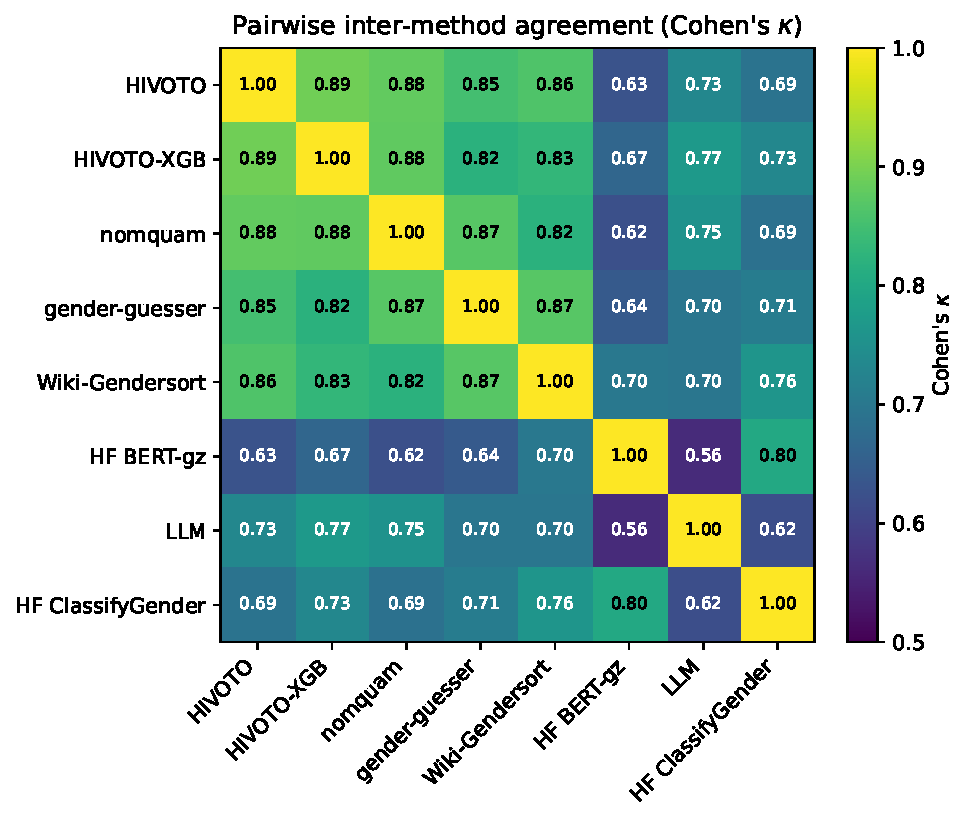
\includegraphics[width=0.85\linewidth]{figures/kappa_heatmap.pdf}
  \caption{Pairwise inter-method agreement (Cohen's $\kappa$) on the \textit{schleiermacher digital} register. GND and the parenthetical-qualifier rule are excluded because their coverage overlap with the name-based methods is too small for a stable pairwise estimate.}
  \label{fig:kappa-heatmap}
\end{figure}


\subsubsection{Per record} For editorial triage we need to know on which entries the methods disagree. For each register entry we record the share of methods that voted for the winning label and sort the entry into one of six tiers: \texttt{unanimous}, \texttt{strong\_majority}, \texttt{weak\_majority}, \texttt{no\_con}-\texttt{sensus}, \texttt{single\_rater}, \texttt{no\_answer}.
The distribution is heavily right-skewed: of $8{,}277$ entries, $4{,}441$ ($53.7\%$) are \texttt{unanimous} and a further $2{,}982$ ($36.0\%$) reach \texttt{strong\_majority}, while $854$ ($10.3\%$) fall into \texttt{weak\_majority} or \texttt{no\_consensus} --- the entries the review interface surfaces first. The breakdown by majority label (Table~\ref{tab:tier-by-label}) reveals a systematic asymmetry between \texttt{male} and \texttt{female} agreement.

For the entries that fall into \texttt{no\_consensus} and \texttt{weak\_majority}, manual inspection of the most-contested records shows that disagreement clusters around four recurring profiles:

\begin{enumerate}
  \item Institutional names mis-parsed as personal names (\eg{} corporate correspondents).
  \item Initials-only entries, where dictionary methods have nothing to match against.
  \item Non-German names lying outside the coverage of the dictionary-based classifiers.
  \item Historically ambiguous names whose gendered usage shifted between the eighteenth and twenty-first centuries --- a problem that modern training data inherently amplifies.
\end{enumerate}

These are precisely the entries flagged for editorial review: disagreement functions as a triage signal, directing editor attention to cases where automated annotation is least reliable.

\begin{table}[h]
  \centering
  \small
  \begin{tabular}{lrrrrr}
    \toprule
    Majority label & $N$ & unanimous & strong\_maj. & weak\_maj. & no\_consensus \\
    \midrule
    \texttt{male}      & $4{,}548$ & $3{,}677$ ($80.8\%$) & $524$ ($11.5\%$) & $216$ ($4.7\%$) & $131$ ($2.9\%$) \\
    \texttt{female}    & $1{,}346$ & $764$ ($56.8\%$)     & $314$ ($23.3\%$) & $213$ ($15.8\%$) & $55$ ($4.1\%$)  \\
    \texttt{ambiguous} & $240$     & $0$ ($0.0\%$)        & $5$ ($2.1\%$)    & $59$ ($24.6\%$)  & $176$ ($73.3\%$) \\
    \bottomrule
  \end{tabular}
  \caption{Per-record agreement tier broken down by the majority label. The methods agree much more readily on \texttt{male} than on \texttt{female}; entries pushed to \texttt{ambiguous} are never unanimous and dominate the editorial review queue. (The remaining $2{,}143$ entries with $n_{\text{answered}} \le 1$ fall into \texttt{single\_rater} or \texttt{no\_answer} and are omitted.)}
  \label{tab:tier-by-label}
\end{table}



Of the $8{,}277$ entries in the register $6{,}934$ ($83,8\%$) reach the \texttt{high} certainty tier through majority agreement or an authority override (Table~\ref{tab:cert-tiers}).  $854$ ($10.3\%$) fall into the \texttt{weak\_majority} or \texttt{no\_consensus} tiers and were flagged for editorial review. 


The agreement tiers described in \S\ref{sec:agreement} map onto the TEI \texttt{@cert} values, but not one-to-one. \texttt{Unanimous} and \texttt{strong\_majority} entries, as well as any entry where an authority override fired, are promoted to \texttt{high}. \texttt{weak\_majority} maps to \texttt{low}, \texttt{no_consensus} to \texttt{contested}. The \texttt{single_rater} tier splits depending on the LLM's self-reported confidence: entries where the LLM committed with high confidence become \texttt{single}, those with low or uncertain self-confidence become \texttt{uncertain}.

\begin{table}[h]
  \centering
  \small
  \begin{tabular}{lrr}
    \toprule
    \texttt{@cert} tier & Entries & Share \\
    \midrule
    \texttt{high}      & $6{,}934$ & $83.8\%$ \\
    \texttt{single}    & $710$     & $8.6\%$  \\
    \texttt{uncertain} & $338$     & $4.1\%$  \\
    \texttt{low}       & $257$     & $3.1\%$  \\
    \texttt{contested} & $38$      & $0.5\%$  \\
    \bottomrule
  \end{tabular}
  \caption{Distribution of the combined certainty tier across the Schleiermacher register ($N = 8{,}277$).}
  \label{tab:cert-tiers}
\end{table}

Manual inspection of the most-contested records shows that disagreement clusters around four recurring profiles: relational naming conventions where the entry's forename field contains the name of a related person rather than the individual themselves; title-only entries without a usable forename; initials-only entries where dictionary methods have nothing to match against; and institutional names mis-parsed as personal names.


A large number of the disagreement is rooted in the data available in the register. Some entities are only listed by their relation to another entity, with the relation encoded in parenthesis, \eg{~\emph{(Frau des \textbf{Heinrich})}, \emph{(Mutter der \textbf{Antonie})}, \emph{(Mann der \textbf{Marianne})}}, as the entry's own forename. This caused the strictly forename-based methods to mislabel the entries and was addressed using the parenthetical-qualifier rule to check for these particles during aggregation.

\begin{table}[h]
  \centering
  \scriptsize
  \setlength{\tabcolsep}{3pt}
  \begin{tabular}{p{0.10\linewidth} p{0.22\linewidth} p{0.30\linewidth} p{0.30\linewidth}}
    \toprule
    xml:id & Entry / note & Vote pattern & Combined \\
    \midrule
    \texttt{S0001932} &
      \textit{Frölich, (Frau des Heinrich)} \newline
      ``Frau des Heinrich Frölich" &
      6 of 7 name-based methods read ``Heinrich" as a forename and return \texttt{male} (\textsc{hfgc}, \textsc{hfg}, \textsc{hv}, \textsc{nqg}, \textsc{wgs}, \textsc{xgb} abstain); the parenthetical-qualifier rule fires on ``Frau des" $\rightarrow$ \texttt{female}; LLM $\rightarrow$ \texttt{female} from the note. &
      \texttt{female} (cert \texttt{high}; LLM\,+\,rule outvote name-based cluster) \\
    \addlinespace
    \texttt{S0001502} &
      \textit{Canitz, Baronin von} \newline
      (no biographical note) &
      Title-only entry without forename; the name-based methods scatter ($\textsc{hfgc},\textsc{hfg},\textsc{xgb}\rightarrow$ \texttt{male}; $\textsc{nqg}\rightarrow$ \texttt{female}; \textsc{gg}, \textsc{hv}, \textsc{wgs} ambiguous); LLM $\rightarrow$ \texttt{female} via German title morphology (\emph{Baronin}). &
      \texttt{female} (cert \texttt{single}; LLM-only resolution) \\
    \addlinespace
    \texttt{S0001317} &
      \textit{Bing, A.\,H.} \newline
      ``Arzt in Berlin" &
      Six of eight methods abstain or return ambiguous because ``A.\,H." is unparseable as a forename; only \textsc{hfgc}, \textsc{hfg}, \textsc{xgb}, and the LLM commit, all to \texttt{male}, the LLM via the masculine ``Arzt". &
      \texttt{male} (cert \texttt{high}; thin but unanimous) \\
    \addlinespace
    \texttt{S9437075} &
      \textit{Fournier, L. und Compagnie} \newline
      ``wohnhaft in der Friedrichsgracht 50" &
      Trading firm; name-based methods read ``L."~as a forename and split (\textsc{hfgc}, \textsc{xgb} $\rightarrow$ \texttt{female}; \textsc{hfg} $\rightarrow$ \texttt{male}; rest ambiguous); only the LLM flags the entry as an institution. &
      \texttt{institution} (cert \texttt{single}; LLM-only resolution) \\
    \bottomrule
  \end{tabular}
  \caption{Examples for the four dominant disagreement types marked for editorial review ($N = 854$ contested entries). Vote patterns are taken from the per-method results.}
  \label{tab:disagreement-examples}
\end{table}

On the Schleiermacher register, the resulting tier distribution is heavily concentrated at \texttt{high} (Table~\ref{tab:cert-tiers}): $6{,}934$ entries ($83.8\%$) reach the high-confidence tier through majority agreement or an authority override, while only $295$ entries ($3.6\%$) fall into the genuinely problematic \texttt{low} or \texttt{contested} tiers. The remaining $1{,}048$ entries ($12.7\%$) are LLM-only cases (\texttt{single} / \texttt{uncertain}) --- entries on which only the LLM, with its full biographical context, was able to commit to a label.


\subsection{Errors in authority data}
In a very small number of cases the existing data seemingly contained ambiguities. These issues surfaced only at the aggregation step of the data enrichment, and helped validating the approach (see Table~\ref{tab:contested-examples}).

\begin{table}[h]
  \centering
  \scriptsize
  \setlength{\tabcolsep}{4pt}
  \renewcommand{\arraystretch}{1.2}
  \begin{tabular}{@{}lp{36mm}cccp{38mm}@{}}
    \toprule
    \texttt{xml:id} & Name & GND & LLM & Combined & Verdict \\
    \midrule
    \texttt{S9145415} &
    Klein, Auguste Ernestine Aemilie (``Tochter des Ernst Ferdinand Klein'') &
    \texttt{male} & \texttt{female} & \texttt{female} (\texttt{cert=high}) &
    GND link resolves to wrong person; aggregator correctly overrode it \\
    \addlinespace
    \texttt{S3729958} &
    Magnus, Leopold (``Portrait- und Genremalerin in Berlin'') &
    \texttt{male} & \texttt{female} & \texttt{male} &
    Note erroneously feminises \emph{Maler} as \emph{Malerin} \\
    \addlinespace
    \texttt{S0003113} &
    O'Bern, Marcus Phillip Ludwig de (``französisch-reformierter\-Prediger\-in\-Halle'') &
    \texttt{male} & \texttt{female} & \texttt{male} &
    LLM was misled by a typo from concatenation: \emph{Prediger in} as \emph{Predigerin} \\
    \bottomrule
  \end{tabular}
  \caption{Three cases of errors in data sources deemed authoritative.}
  \label{tab:contested-examples}
\end{table}

The first case, \texttt{S9145415}, is a mislinked authority reference: the register entry refers to Auguste Ernestine Aemilie Klein, daughter of Ernst Ferdinand Klein, but the editorial GND link resolves to a different person, Auguste Klein (1777--), a male painter and writer active in Rome, whose authority record correctly carries \texttt{male}. The dictionary methods, the parenthetical-qualifier rule, and the LLM all return \texttt{female}; the aggregator promotes \texttt{female} to \texttt{cert=high} and overrides the mislinked GND signal.

The other two cases are errors in the editorial biographical notes that mislead the LLM. In \texttt{S3729958}, the note ``Portrait- und Genremalerin in Berlin'' should read \emph{Genremaler}; the feminine suffix \emph{-in} cues the LLM to \texttt{female}. In \texttt{S0003113}, a missing space concatenates \emph{Prediger in Halle} into \emph{Predigerin Halle} and produces the same misreading. In both cases the name-based methods resist, the majority outvotes the LLM, and the combined label remains \texttt{male}.

TODO: Tabelle raus?

\begin{table}[tb]
\centering
\small
\setlength\tabcolsep{4pt}
\begin{tabular}{llrrrll}
\toprule
Family & Method & Coverage\,(\%) & Binary labels\,(\%) & Accuracy on GND\,(\%)\\
\midrule
Authority & GND & 27.2 & 27.2 & ---\\
\midrule
\multirow Dictionary & gender-guesser & 74.1 & 67.7 & 99.5\\
 & HIVOTO & 74.1 & 70.3 & 100.0\\
 & Wiki-Gendersort & 73.4 & 69.5 & 99.5\\
\midrule
\multirow Probabilistic & NQG & 74.1 & 69.6 & 100.0 \\
 & HIVOTO-XGBoost$^\dagger$ & 72.9 & 72.5 & 99.2 \\
\midrule
\multirow Transformer & HF ClassifyGender & 74.1 & 68.7 & 98.6 \\
 & HF Genderize & 74.1 & 67.4 & 98.3  \\
\midrule
LLM & gpt-oss:20b & 100.0 & 88.5 & 99.9 \\
\bottomrule
\end{tabular}
\caption{Classification methods in the genderTagger pipeline, evaluated on the \textit{schleiermacher digital} person register
($n=8{,}277$ entries; ground-truth subset: GND-verified records with binary gender, $n=2{,}253$).
\emph{Coverage}: share of all entries on which the method returned any non-abstention label.
\emph{Binary labels}: share classified specifically as \texttt{male} or \texttt{female}; the gap to \emph{Coverage}\ reflects ambiguous, conflicting, \texttt{unknown}, or \texttt{organisation} outputs.
\emph{Accuracy on GND}: share of correct predictions on the ground-truth subset.
$\dagger$~HIVOTO-XGBoost is experimental and excluded from the combined vote.}
\label{tab:methods}
\end{table}


% Acknowledgements for colleagues, referees, ...
% ==============================================
\begin{acknowledge}
KD acknowledges support by DFG Project \geprislink{000000000}.
\end{acknowledge}

\begin{data}
My data is publicly available on zenodo.
\end{data}

\begin{aiuse}
No AI hallucinations over here.
\end{aiuse}

% Bibliography with BibTeX
% ========================
\bibliographystyle{eceasst}
\bibliography{gendertagger}

\end{document}
